\documentclass{implementierungsheft}
% glossary
\makeglossaries

\begin{document}
\newglossaryentry{label}{
    name=Label,
    plural=Labels,
    description={Rezepte können mit bezeichnenden Stichwörtern, sogenannten Labels, versehen werden. Dies ermöglicht das Filtern von Rezepten nach bestimmten Eigenschaften (z.B. vegetarisch, glutenfrei, halal)}
}
\maketitle
\tableofcontents
\newpage

\section*{Gender-Hinweis}
Zur besseren Lesbarkeit wird in diesem Entwurfsheft das generische Maskulinum verwendet.
Die in diesem Heft verwendeten Personenbezeichnungen beziehen sich - sofern nicht anders kenntlich gemacht - auf alle Geschlechter.
\newpage

\section{Umsetzung der Zielbestimmungen des Pflichtenhefts}
Es wurden alle Muss-, Soll- und Kannkriterien umgesetzt. Die Applikation wurde um die Folgenden Features erweitert:
\begin{itemize}
    \item An sinnvollen Stellen wurden zusätzliche Pop-Up-Fenster eingefügt, die z.B. nach Bestätigung einer Aktion fragen.
    \item Es gibt eine weitere Ansicht, die die exportierten Rezepte als PDF-Vorschau anzeigt.
\end{itemize}
\newpage
\section{Änderungen am Entwurf}
In den folgenden UML-Diagrammen werden abgeänderte Methoden und Attribute blau markiert, entfernte rot und neue grün.
\subsection{Änderungen an dem Modellayer}
\begin{figure}[htp]
    \centering
    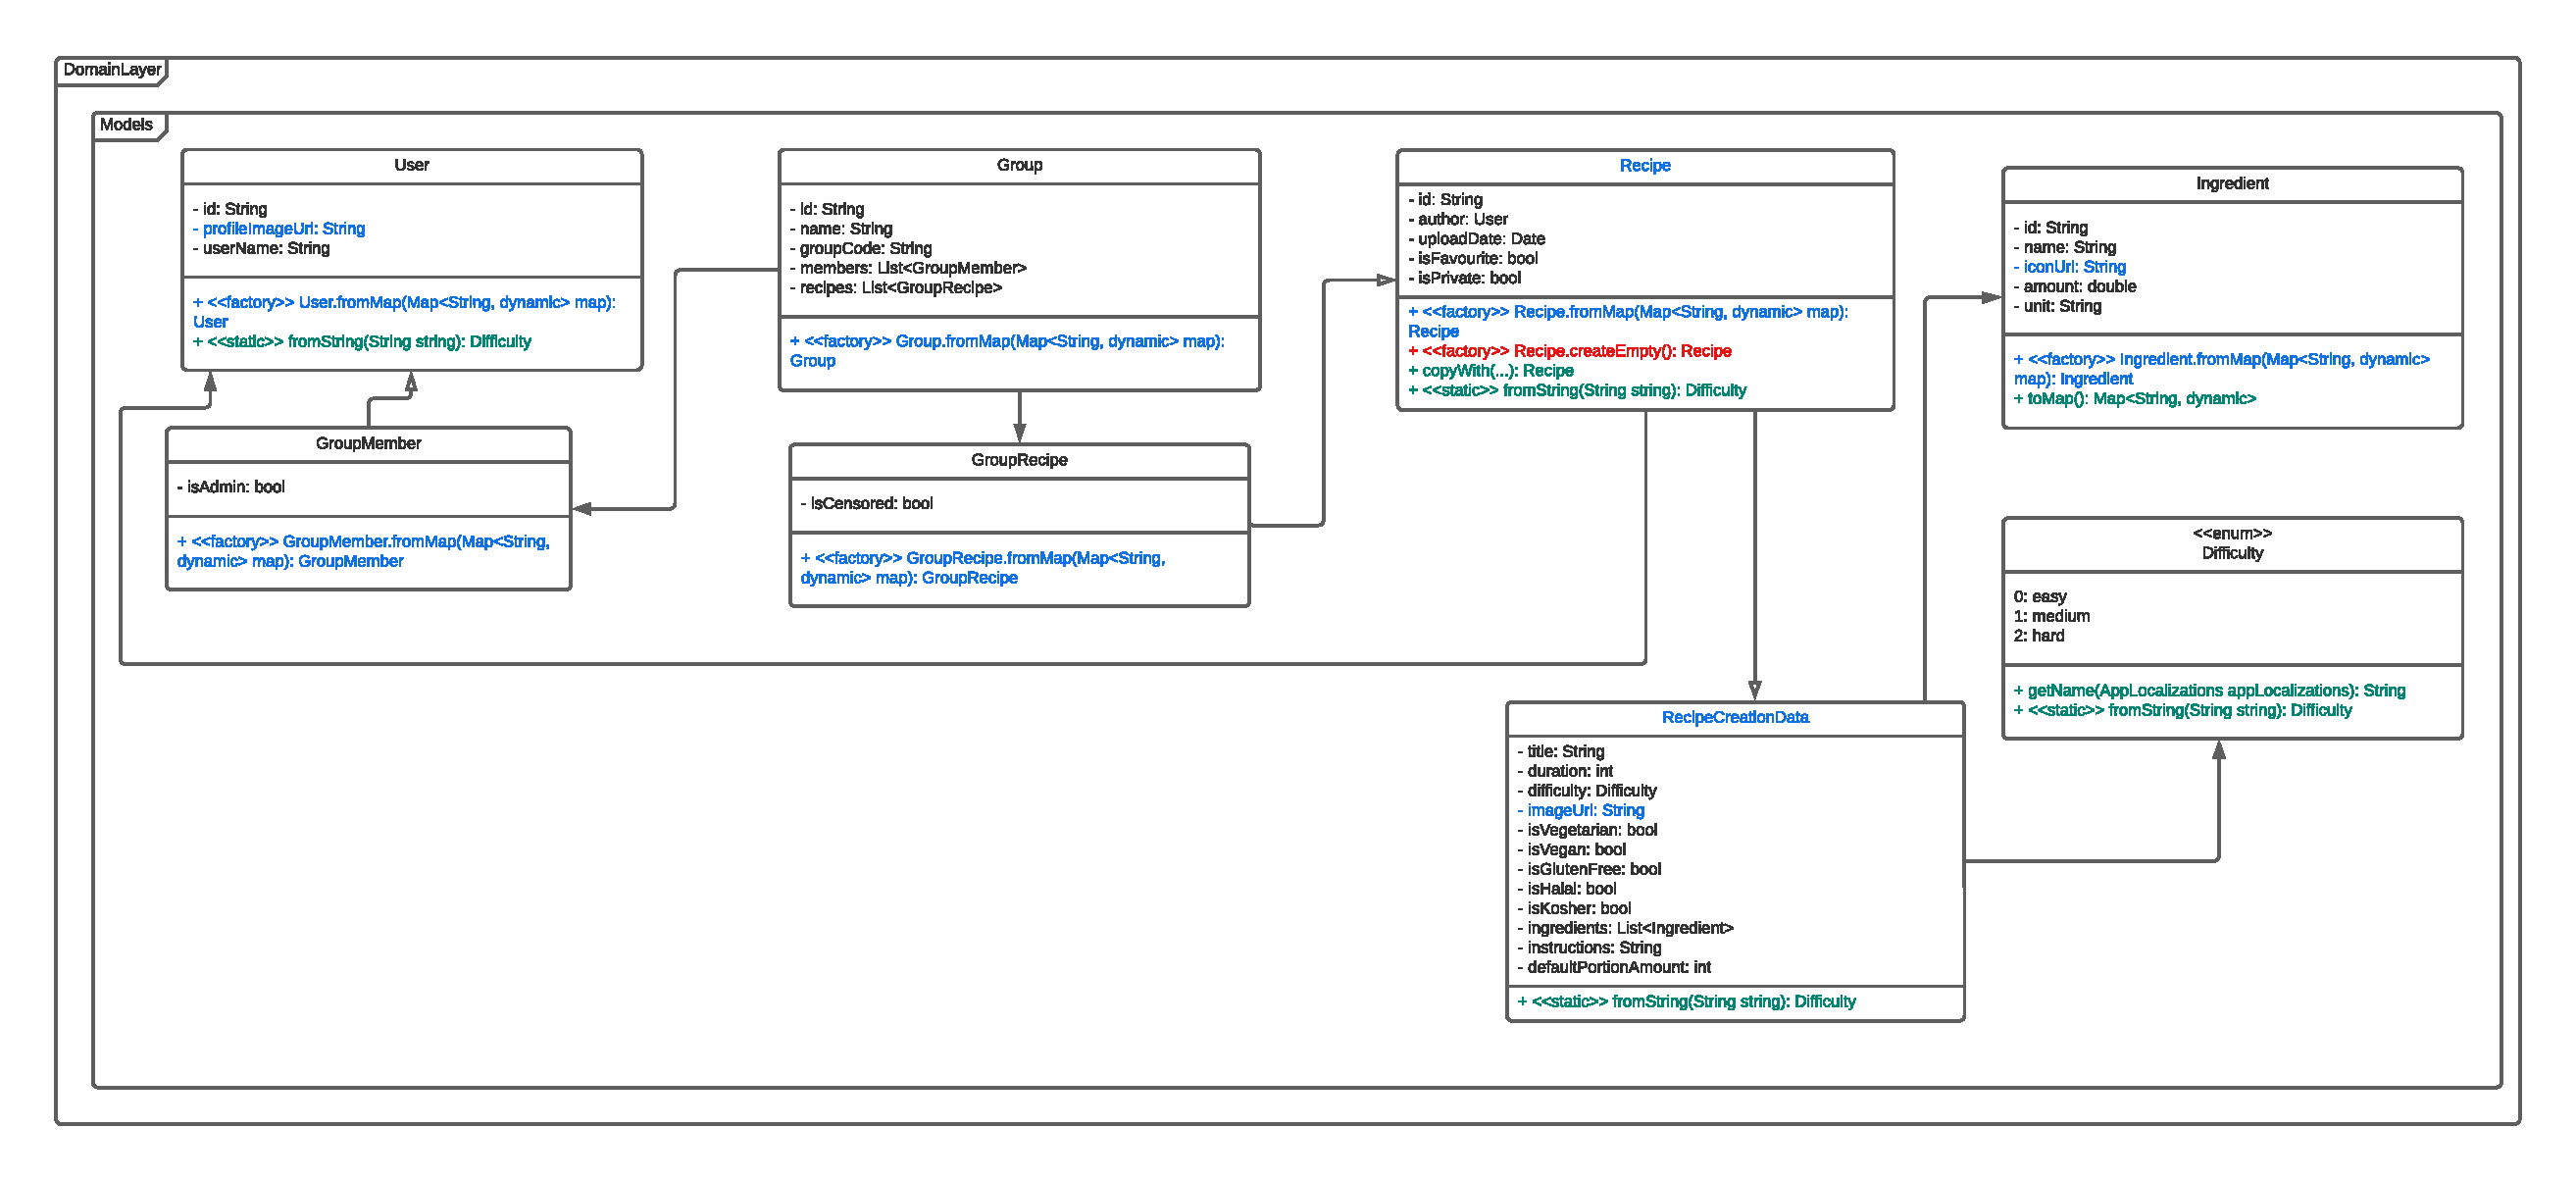
\includegraphics[width=0.95\textwidth]{images/uml/modellayer.pdf}
    \caption{Änderungen am Modellayer}
    \label{fig:modellayer}
\end{figure}
\paragraph*{\texttt{fromMap(Map<String, dynamic> map)}} Die Factory-Methoden \texttt{fromJson} wurden in \texttt{fromMap} umbenannt, da sie unabhängig von der Serialisierungsmethode sind.
\paragraph*{\texttt{toMap()}} Die statische Methode \texttt{toMap} wurde bei einigen Klassen hinzugefügt, um die Serialisierung zu vereinfachen. Sie gibt ein \texttt{Map<String, dynamic>} zurück, das die Attribute der Klasse enthält.
\paragraph{\texttt{Recipe.copyWith(...)}} Die Methode \texttt{copyWith} wurde hinzugefügt, um ein Rezept zu kopieren und dabei einzelne Attribute zu ändern. Die zuändernden Attribute werden als benannte Parameter übergeben.
\newpage
\section{Glossar}
\printglossary[style=altlist]
\end{document}